\chapter{DHTML}
\section{Definizione}
DHTML non è un linguaggio specifico, ma l'integrazione di \texttt{HTML, CSS, JS e DOM} per rendere una pagina interattiva e dinamica lato client.

\begin{figure}[H]
    \centering
    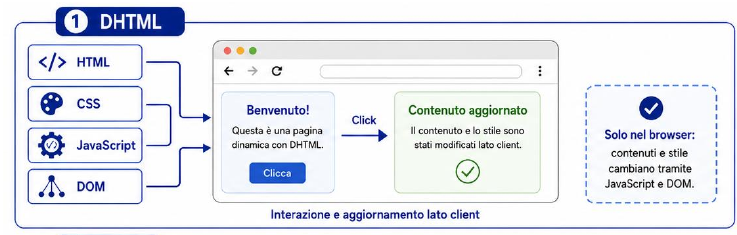
\includegraphics[scale=0.8]{figures/file incollato.png}
\end{figure}

Questa nuova struttura permette di aggiornare il contenuto senza ricaricare la pagina, reagire agli eventi utente, modificare stile e struttura del documento, costrutire interfacce più ricche e reattive

\section{Componenti principali}
\begin{itemize}
    \item \texttt{\textbf{HTML}}: Struttura dei contenuti
    \item \texttt{\textbf{CSS}}: Presentazione e stile
    \item \texttt{\textbf{JS}}: Comportamento e logica
    \item \texttt{\textbf{DOM}}: Accesso e manipolazione degli elementi della pgina
\end{itemize}

\newpage
\section{Struttura di una pagina HTML5}
Una pagina HTML5 ben formata ha una struttura minima fissa.

Lo scheletro è composto da 4 elementi annidati.
\begin{tcolorbox}[breakable, title={Esempio pagina HTML5}]
\begin{lstlisting}[language=HTML]
<!DOCTYPE html>
<html lang="it">
<head>
  <meta charset="UTF-8">
  <title>Pagina di esempio</title>
</head>
<body>
  <!-- contenuto, UI, input/output -->
  <script src="app.js" defer></script>
</body>
</html>
\end{lstlisting}
\end{tcolorbox}
\subsection{Best practice}
\begin{itemize}
    \item Il codice JS in file esterni, incluso con defer: il browser scarica lo script in parallelo all'HTML e lo esegue dopo il parsing
    \item In alternativa \texttt{type="module"} per usare i moduli
\end{itemize}

\chapter{AJAX}
\section{Limite di DHTML}
Può modificare contenuti e stile nel browser, ma da solo non introduce un meccanismo strutturato di comunicazione asincrona con il server
\section{Definizione}
È un pattern utilizzato per creare applicazioni Web interattive
\begin{figure}[H]
    \centering
    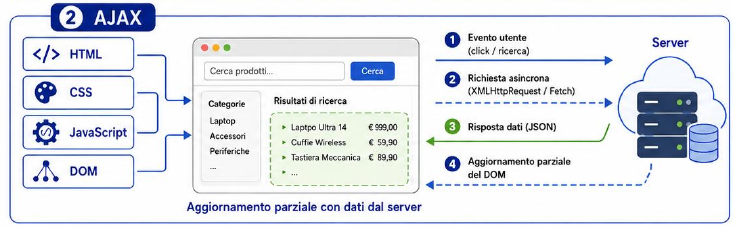
\includegraphics[scale=0.8]{figures/Schermata_20260601_121706}
\end{figure}

\section{Componenti}
\begin{itemize}
    \item \textbf{HTML e CSS}: Struttura e presentazione
    \item \textbf{Document Object Model (DOM)}: Rappresentazione ad albero della pagina, navigabile e modificabile da codice per aggiornamenti dinamici
    \item \textbf{XML e XSLT}: Formato originario per scambio e trasformazione dei dati tra client e server
    \item \textbf{Javascript}: Il "collante" che orchestra eventi, DOM e richieste XHR
\end{itemize}

\subsection{AJAX come estensione di DHTML}
AJAX aggiunge richieste asincrone (\texttt{XMLHttpRequest o Fetch}) verso il server, riceve i dati (oggi tipicamente JSON) e aggiorna solo una parte della pagina senza ricaricarla
\subsection{Cosa abilita?}
\begin{itemize}
    \item Aggiornamento parziale della pagina (solo i dati che cambiano)
    \item Interfacce reattive, vicine all'esperienza desktop (rich UI)
    \item Riduzione del traffico di rete e dei tempi di attesa
\end{itemize}
\section{WEB 2.0}
AJAX è la tecnologia abilitante del \textbf{Web 2.0}
\subsection{I 6 principi del Web 2.0}
\begin{itemize}
    \item \textbf{Il Web come piattaforma}: le applicazioni vivono nel browser, non sul desktop
    \item \textbf{Intelligenza collettiva}: Il valore cresce con il contributo degli utenti
    \item \textbf{Al di sopra del singolo dispositivo}: Servizi accessibili da qualsiasi client
    \item \textbf{I dati sono il nuovo "Intel Inside}: Il vantaggio competitivo sta nei dati gestiti
    \item \textbf{Esperienze utente ricche}: Interfacce reattive grazie ad AJAX
\end{itemize}
\section{Utilizzi di AJAX}
\begin{itemize}
    \item \textbf{Valdizione in tempo reale dei form}
    \item \textbf{Auto-completamento}
    \item \textbf{Operazioni master-detail}
    \item \textbf{Aggiornamento incrementale e live update}
\end{itemize}

\newpage
\section{Archiettura Web con AJAX}
\subsection{Architettura Web Classica}
\begin{figure}[H]
    \centering
    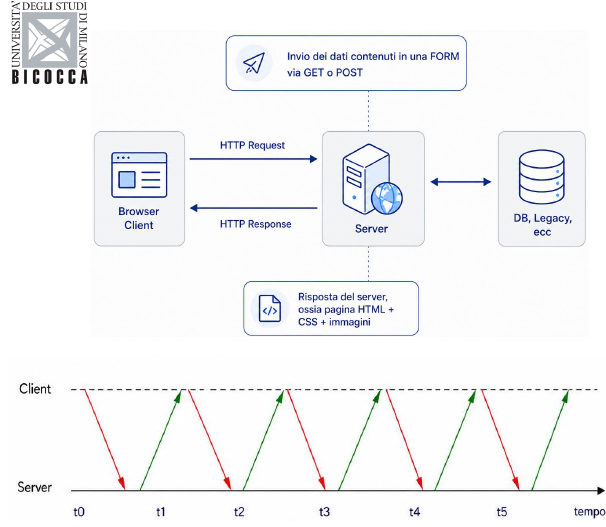
\includegraphics[scale=0.65]{figures/Schermata_20260601_123931.png}
\end{figure}
\begin{itemize}
    \item \textbf{Ciclo richiesta/risposta}

    Il browser invia una richiesta HTTP.

    Il server interroga il database e restituisce un'intera pagina HTML con CSS e immagini.

    \item \textbf{Andamento nel tempo}

    Ogni interazione produce un ciclo completo Request $\to$ Response.

    Il client resta bloccato in attesa: l'utente non può fare altro finchè la pagina non si è ricaricata.

    \item \textbf{Risultato}

    Esperienza utente discontinua e traffico di rete sproporzionata rispetto all'informazione effettivamente nuova.
\end{itemize}

\subsection{Architettura Web con AJAX}
\begin{figure}[H]
    \centering
    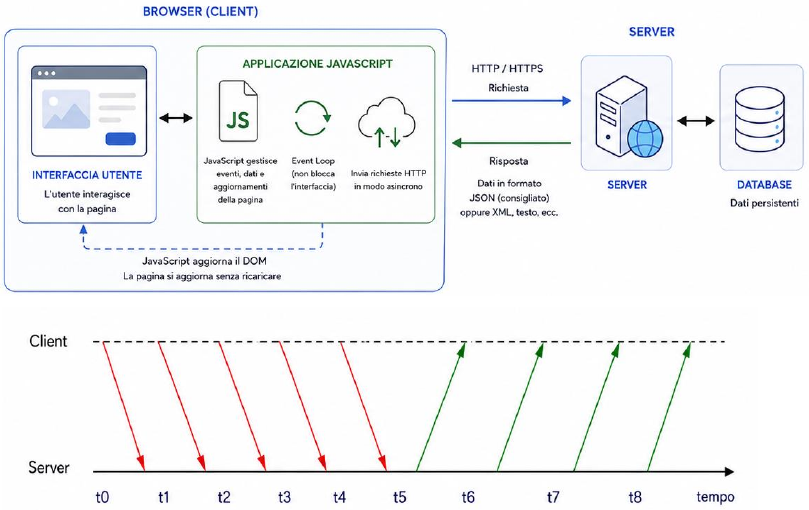
\includegraphics[scale=0.65]{figures/Schermata_20260601_124615.png}
\end{figure}
\begin{itemize}
    \item \textbf{AJAX come intermediario}

    Tra l'interfaccia utente e il server si inserisce un motore JS: l'UI dialoga con l'engine in locale (HTML + CSS), l'engine parla col server in HTTP scambiando solo dati (XML o JSON)

    \item \textbf{Asincrono}

    Più richieste possono essere inviate senza attendere le risposte.

    L'utente può continuare ad interagire mentre le risposte arrivano quando sono pronte e solo i dati necessari vengono aggiornati nella pagina.
\end{itemize}

\section{Trasmissione dei dati}
Lo scambio di dati tra client e server è il punto critico delle applicazioni web interattive: dimensioni del payload, parsing e compatibilità influenzando direttamente le presentazioni percepite.

\newpage
\section{Confronto modelli di esecuizione}
Tre paradigmi differenti rispetto a chi guida il flusso di controllo e quando il programma termina

\subsection{Sequenziale}
\subsubsection{Flusso}
\begin{enumerate}
    \item Il programma decide cosa fare e quando farlo
    \item Esegue input $\to$ elabora $\to$ output $\to$ termina
\end{enumerate}
\subsubsection{Caratteristiche}
\begin{itemize}
    \item Terminazione esplicita
    \item Nessuna interazione durante l'esecuzione
\end{itemize}
\subsubsection{Esempi}
\begin{itemize}
    \item Compilatore
    \item Script di build
    \item job batch
\end{itemize}

\subsection{Interattivo}
\subsubsection{Flusso}
\begin{enumerate}
    \item Il programma chiede input, attende, elabora
    \item L'utente risponde a richieste predefinite 
\end{enumerate}
\subsubsection{Caratteristiche}
\begin{itemize}
    \item Controllo guidato dal programma
    \item Sequenza prevedibile di passi
\end{itemize}
\subsubsection{Esempi}
\begin{itemize}
    \item CLI a prompt
    \item wizard
    \item REPL
\end{itemize}
\subsection{Reattivo (event-driven)}
\subsubsection{Flusso}
\begin{enumerate}
    \item Il programma reagisce a eventi esterni
    \item Resta in attesa, non termina
\end{enumerate}
\subsubsection{Caratteristiche}
\begin{itemize}
    \item Controllo guidato dall'ambiente
    \item Asincrono, non deterministico
\end{itemize}
\subsubsection{Esempi}
\begin{itemize}
    \item GUI
    \item Pagine web
    \item Server
    \item Embedded
\end{itemize}

\newpage
\section{Sistemi reattivi}
\subsection{Definizione}
Un sistema reattivo mantiene un interazione continua con il suo ambiente, rispondendo a stimoli esterni con tempi e modalità dettati dall'ambiente stesso.
\begin{figure}[H]
    \centering
    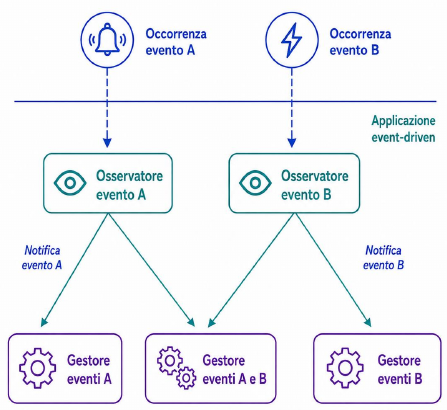
\includegraphics[scale=0.8]{figures/Schermata_20260603_103043.png}
\end{figure}

\subsection{Caratteristiche}
\begin{itemize}
    \item \textbf{Non-terminazione}: Il sistema resta vivo, in attesa del prossimo evento
    \item \textbf{Asincronia}: Gli eventi arrivano in tempi non prevedibili a priori
    \item \textbf{Concorrenza}: Più sorgenti di eventi attive simultaneamente
\end{itemize}

Non è possibile identificare staticamente un flusso di controllo unitario, il programma pricnipale si limita a inizializzare l'applicazione, istanziando gli osservatori e associandovi gli opportuni handler.
Questa associazione può essere dinamica.

\subsection{Modello di esecuzione}
\begin{itemize}
    \item \textbf{Single-threaded}(in JS): Un solo handler alla volta
    \item \textbf{Run-to-completion}: Ogni handler termina prima del successivo
    \item \textbf{Conseguenza}: Handler lunghi bloccano l'intera UI
\end{itemize}

\newpage
\section{Formati e protocolli AJAX}
\begin{itemize}
    \item \textbf{JSON}: standard de-facto, compatto, parsing nativo nel browser
    \item \textbf{REST + JSON}: pattern dominante per le API web moderne
    \item \textbf{GrapQL}: alternativa che permette al client di richiedere solo i campi che gli servono
    \item \textbf{XML}: formato originario di AJAX, oggi raro nelle web app ma diffuso in contesti enterprise
    \item \textbf{SOAP e XML-RPC}: storici, sopravviviono in ambito legacy
\end{itemize}

\section{Criticità di AJAX}
\subsection{Navigazione e bookmark}
\begin{itemize}
    \item Il tasto "back" e i preferiti registrano cambi di URL: con AJAX la pagina cambia contenuto senza cambiare URL, e l'utente perde il riferimento allo stato
    \item Mitigato dalla History API, permette di aggiornare URL e cronologia senza ricaricare
\end{itemize}
\subsection{Indicizzazione e SEO}
\begin{itemize}
    \item I contenuti caricati via AJAX possono non essere indicizzatti, storicamente i crawler non eseguivano JS, oggi lo fanno ma con limiti
    \item Soluzioni moderne: Server-Side Rendering e idratazione
\end{itemize}
\subsection{Complessità del client}
\begin{itemize}
    \item La logica si sposta sul client, il bundle JS cresce, allungando il tempo di first load
    \item Debug più difficile, la stessa logica è distribuita tra client e server
\end{itemize}
\subsection{Pressione sul server}
\begin{itemize}
    \item AJAX rende facile fare richieste piccole e frequenti, l'effetto cumulativo può pesare più del singolo full reload
\end{itemize}

\chapter{XMLHttpRequest - Interazione server AJAX}
\section{Cos'è?}
È un API JS fornita da tutti i browser moderni per inviare richieste HTTP e ricevere risposte \uline{senza ricaricare la pagine}.

\section{Cosa offre?}
\begin{itemize}
    \item \textbf{Modello asincrono}: La richiesta non blocca la UI, alla risposta scatta un evento.
    \item \textbf{Ciclo di vita esposto}: La proprietà \texttt{readyState} indica a che punto è la richiesta.
    \item \textbf{API a callback}: Si registra un handler su \textsl{onreadystatechange} che reagisce ai cambiamenti di stato.
\end{itemize}

\section{Metodi principali}
\begin{tabularx}{\linewidth}{|l|X|}
    \hline
    \textbf{Metodo} & \textbf{Cosa fa} \\
    \hline
    new \texttt{XMLHttpRequest()} & Crea l'oggetto richiesta \\
    \hline
    \texttt{setRequestHeader(k, v)} & Aggiunge un header HTTP (es. Content-Type) \\
    \hline
    \texttt{send(body)} & Invia la richiesta body = null per GET \\
    \hline
    \texttt{abort()} & Interrompe una richiesta in corso \\
    \hline
    \texttt{getResponseHeader(name)} & Legge un header HTTP della risposta \\
    \hline
\end{tabularx}
\subsection{Schema d'uso}
\begin{enumerate}
    \item Creare l'oggetto
    \item Registrare \texttt{onreadystatechange}
    \item \texttt{open()} con i parametri
    \item Eventuali \texttt{setRequestHeader}
    \item \texttt{send()}
\end{enumerate}

\texttt{setRequestHeader} serve quando si invia un POST con dati form: imposta header HTTP come Content-Type prima di \texttt{send()}

\section{Proprieà di interesse}
\begin{tabularx}{\linewidth}{|l|X|}
    \hline
    \textbf{Proprietà} & \textbf{Significato} \\
    \hline
    \texttt{readyState} & Stato del ciclo di vita (0-4) \\
    \hline
    \texttt{status} & Codice HTTP della risposta \\
    \hline
    \texttt{responseXML} & Corpo della risposta parsato come DOM XML \\
    \hline
    \texttt{onreadystatechange} & Handler chiamato a ogni cambio di stato  \\
    \hline
    \texttt{statusText} & Descrizione testuale dello status \\
    \hline
\end{tabularx}
\subsection{Sincorno o asincrono}
Il terzo parametro di \texttt{open(method, url, \textbf{async})} sceglie la modalità di esecuzione

\subsubsection{async = true (raccomandato)}
\begin{itemize}
    \item Il browser invia la richiesta e continua a eseguire il resto dello script: la UI resta attiva
    \item La risposta arriverà più tardi: bisogna registrare un handler on \texttt{readystatechange} prima di chiamare \texttt{send()}
\end{itemize}
\subsubsection{async = false (sconsigliato)}
\begin{itemize}
    \item \texttt{send()} blocca il thread JS fino alla risposta: la pagina si congela
    \item Deprecato sul main thread, tutti i browser mostrano un warning, da evitare in produzione
\end{itemize}

\newpage
\section{Ciclo di vita}
Il browser, tramite l'oggetto \texttt{XMLHttpRequest}, attraversa diverse fasi durante la comunicazione con il server.

La proprietà readyState indica in quale fase ci troviamo.

\begin{figure}[H]
    \centering
    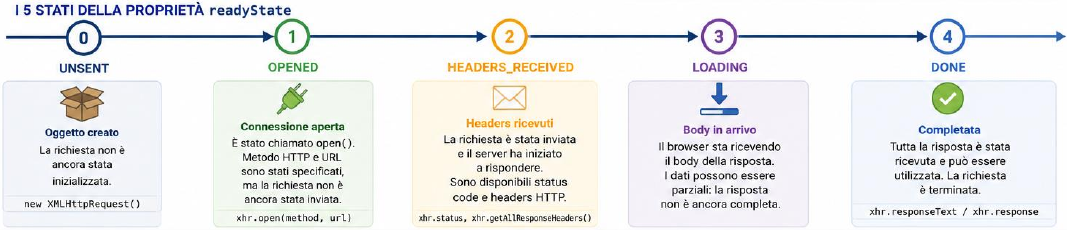
\includegraphics[scale=0.6]{figures/Schermata_20260603_112617.png}
\end{figure}

Il flag che ci interessa è \texttt{readyState == 4} (richiesta completata).

Accoppiato a \texttt{status == 200} indica una risposta utilizabile.

L'evento \texttt{onreadystatechange} viene scatenato a ogni transizione: il nostro handler tipicamente filtra solo lo stato 4

\subsection{Cos'è readyState?}
È una proprietà dell'oggetto \texttt{XMLHttpRequest} che rappresenta lo stato interno della richiesta \texttt{HTTP}.

Viene aggiornata automaticamente dal browser e il suo valore cambia ogni volta che la richiesta avanza in una nuova fase.

\subsection{L'evento readystatechange}
Ogni volta che readyState cambia, il browser scatena l'evento readystatechange.

Possiamo intercettarlo per eseguire del codice al momento giusto

\subsection{Risposta del server}
\begin{tabularx}{\linewidth}{|l|X|}
    \hline
    \textbf{Proprietà} & \textbf{Descrizione} \\
    \hline
    \texttt{responseText} & Restituisce i dati della risposta come stringa \\
    \hline
    \texttt{responseXML} &  Restituisce i dati della risposta come XML \\
    \hline
\end{tabularx}

\subsubsection{Proprietà responseText}
\begin{itemize}
    \item Se la risposta dal server non è XML, usare la proprietà responseText
    \item La proprietà responseText restituisce la risposta come stringa
\end{itemize}

\subsubsection{Proprietà responseXML}
\begin{itemize}
    \item Se la risposta dal server è XML e si vuole analizzare come oggetto XML, usare la proprietà responseXML
\end{itemize}

\section{Richieste con fetch() - alternatva moderna e più semplice}
\texttt{fetch()} è l'API moderna per richieste HTTP.

Restituisce una Promise, niente readyState, niente onreadystatechange, è disponibile in tutti i browser moderni e in Node.js dalla 18

\begin{tcblisting}{%
    title={XMLHttpRequest}, 
    breakable, 
    listing only, 
    listing options={%
        language=Java, % Puoi usare JavaScript se configurato nel preambolo
        basicstyle=\small\ttfamily,
        keywordstyle=\color{purple}\bfseries,
        stringstyle=\color{blue},
        commentstyle=\color{gray},
        showstringspaces=false,
        breaklines=true
    }
}
const xhr = new XMLHttpRequest();
xhr.onreadystatechange = function() {
    if (xhr.readyState === 4 && xhr.status === 200) {
        const data = JSON.parse(xhr.responseText);
        use(data);
    }
};
xhr.open("GET", "/api/data", true);
xhr.send();
\end{tcblisting}
\begin{tcblisting}{%
    title={fetch + async/await}, 
    breakable, 
    listing only, 
    listing options={%
        language=Java, 
        basicstyle=\small\ttfamily,
        keywordstyle=\color{purple}\bfseries,
        stringstyle=\color{blue},
        commentstyle=\color{gray},
        showstringspaces=false,
        breaklines=true
    }
}
async function load() {
    try {
        const res = await fetch("/api/data");
        if (!res.ok) throw new Error(res.status);
        const data = await res.json();
        use(data);
    } catch (err) {
        console.error(err);
    }
}
\end{tcblisting}